\documentclass{sig-alternate-05-2015}
\graphicspath{ {./images/} }

\makeatletter
\def\@copyrightspace{\relax}
\makeatother

\begin{document}

\setcopyright{acmcopyright}

\title{Multi-Agent AI}
\subtitle{[Group Coursework 1]}

\numberofauthors{3}
\author{
\alignauthor
Aksel Cakmak\\
       \affaddr{15047472}\\
       \email{zcababc@ucl.ac.uk}
% 2nd. author
\alignauthor
Chong Yang\\
       \affaddr{18089022}\\
       \email{ucabcya@ucl.ac.uk}
% 3rd. author
\alignauthor
Chen Song \\
       \affaddr{17040773}\\
       \email{ucabcs3@ucl.ac.uk}
}

\maketitle

\section{Introduction}


\section{Approach and Result}
Typically, the body of a paper is organized
into a hierarchical structure, with numbered or unnumbered
headings for sections, subsections, sub-subsections, and even
smaller sections.
\footnote{This is the second footnote.}

\subsection{Problem 1: Data Exploration and Literature Review}

\subsection{Problem 2: Basic Bidding Strategy}
In this section, we analyse two basic bidding strategies, which are Constant Bidding Strategy and Random Bidding Strategy, and evaluate their performance based on the number of clicks within a limited budget of 6,250 CNY fen. 
Evaluation function: For the single-agent basic bidding strategies, the main metric to rank the strategies are based on the clicks from winning impressions.

\subsubsection{Constant Bidding Strategy}
In order to find an optimal constant value, we loop the constant bid prices from 0 to 300, which are the minimum bid price and maximum bid price, to find out the bid price with the highest clicks from winning impressions. Specifically, for each constant price, we retrieve the columns of 'payprice' and 'click' for all the bids in the training set. Then we compare our constant bid price with the 'payprice' for each bid and add up the click into our total clicks if our constant bid price is great than or equal to the 'payprice' while the total spend is calculated at the mean time. Afterwards we remove the clicks from bottom to top where the total spend has been over our limited budget.

Analysis: 
Figure 1 shows that how the number of clicks changes based on the increment of the constant bidding price.
The clicks increase dramatically when the constant bidding price increases from 1 to 24 and the climax of clicks is 134 when the constant bidding price is 24. Then the clicks drop sharply when the bidding price increases from 25 to 69. Afterwards, the clicks decrease smoothly.

In order to evaluate our result on validation set, initially we need to normalize the budget based on the Equation 1.\\

\begin{equation}bidPrice_{validation}=\frac{sizeOfValidation}{sizeOfTrain} * bidPrice_{train}\end{equation}


Figure 2 shows the changes of number of clicks depending on bid price in the validation set with a normalized budget. We could see the clicks are relatively high when the bid price is between 18 to 68. Moreover, the highest clicks are 15 while the clicks are 12 when bid price is 24. Therefore, bid price 24 is a relatively satisfactory price in the validation set.

\begin{figure}
\centering
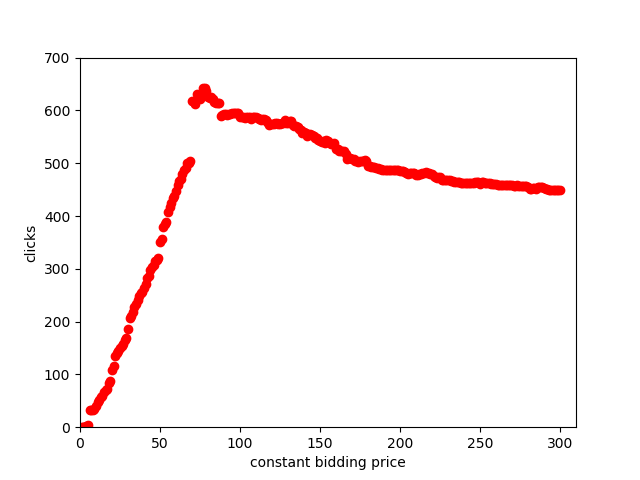
\includegraphics[height=2in, width=2in]{images/constant_bidding.png}
\caption{Validation set - bid price and clicks}
\end{figure}

\begin{figure}
\centering
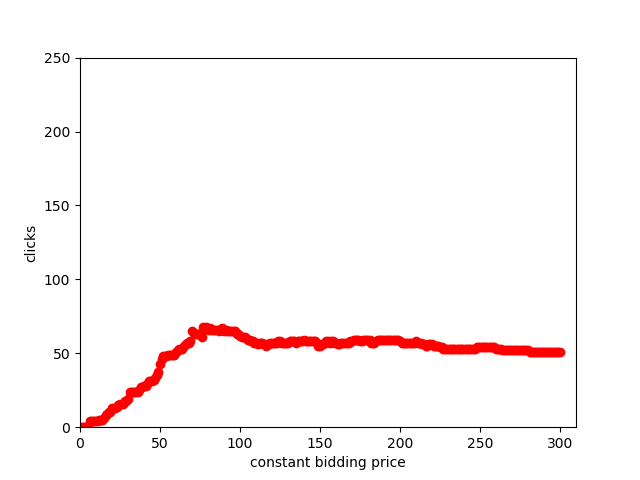
\includegraphics[height=2in, width=2in]{images/constant_bidding_validation.png}
\caption{Validation set - bid price and clicks}
\end{figure}




\subsubsection{Random Bidding Strategy}
In order to find the optimal bidding range for random bidding, we step through a range of lower bound and a range of upper bound to find out the bid price with the highest clicks from winning impressions. Similarly, we use the same method as the one in Constant Bidding Strategy to calculate the clicks. 

Analysis: 
The highest clicks are 132 generated from range(30, 40) and the second highest clicks are 131 generated by range(0, 50) in the training set. By normalizing the budget in the validation set based on equation 1, we find the highest clicks are 15 generated from the range(0, 50). Therefore, the findings in training set successfully match validation set. 

\subsubsection{Competition among homogeneous random bidding agents}

\subsection{Problem 3: Linear Bidding Strategy}
In order to apply CTR estimation to for a linear bidding strategy, we initially retrieve the these features as independent variables X: day, hour, region, ad exchange, slot width, slot height, advertiser, slot visibility, slot format, OS, browser, and slot price from the data set. Specifically, we categorize the slot price to five categories based on the price values, and we extract the OS and browser from the column useragent. And the rest features could be simply fetched from the data. The click from the data is our predictor Y.
Afterwards, we import the Logistic Regression model from sklearn and train the model with the independent variables and predictor from the training set. Then we use the trained model to predict the click of test data and validation data separately. The pCTR of the validation data could be calculated with the equation 2.
\begin{equation}pCTR=\frac{numOfClicks}{numOfWinningImpressions}\end{equation}

The bid price for each bid is calculated as equation 3. As shown in Figure 3, the total clicks increase sharply when base bid increases from 1 to 20 and drop smoothly after then. The value clicks is maximized as 39 when the base bid is 20.

\begin{equation}bidPrice=\frac{baseBidPrice*pCTR}{avgCTR}\end{equation}

\begin{figure}
\centering
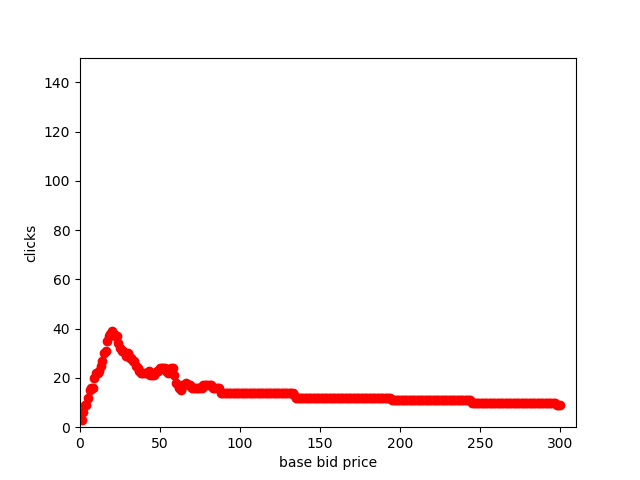
\includegraphics[height=2in, width=2in]{images/base_bid_price.png}
\caption{Validation set - base price and clicks}
\end{figure}

Comparison:
\begin{table}
\centering
\caption{Behavior Comparison}
\begin{tabular}{|c|c|c|l|} \hline
&Constant Bidding&Random Bidding&Linear Bidding\\ \hline
price&24&range(0, 50)&20(base)\\ \hline
clicks&12& 15&39\\
\hline\end{tabular}
\end{table}

Obviously, the behavior of the linear bidding strategy is much better than random bidding and constant bidding strategies. The optimal value of clicks in linear bidding is 39 while the ones of constant bidding and random bidding are merely 12 and 15 separately.

\subsection{Problem 4: Non-Linear Bidding Strategy}
We calculate the non-linear bidding price based on ORTB (equation 4), and we step through some combination of c and lamda to find the optimal pair generating the optimal bid prices. We find the value of clicks is 39 when c equals to 39 and lamda equals to 1.31072e-05. Therefore, our non-linear bidding strategy just generates the same result as linear bidding strategy.
\begin{equation}bidPrice=\sqrt{\frac{c}{\lambda} * pCTR + c^2} - c\end{equation}

\subsection{Problem 5: Multiagent Bidding Strategy}

\section{Conclusions}
This paragraph will end the body of this sample document.
Remember that you might still have Acknowledgments or
Appendices; brief samples of these
follow.




\section{sample format}

\subsubsection{Inline (In-text) Equations}
A formula that appears in the running text is called an
inline or in-text formula.  It is produced by the
\textbf{math} environment, which can be
invoked with the usual \texttt{{\char'134}begin. . .{\char'134}end}
construction or with the short form \texttt{\$. . .\$}. You
can use any of the symbols and structures,
from $\alpha$ to $\omega$, available in
\LaTeX\cite{Lamport:LaTeX}; this section will simply show a
few examples of in-text equations in context. Notice how
this equation: \begin{math}\lim_{n\rightarrow \infty}x=0\end{math},
set here in in-line math style, looks slightly different when
set in display style.  (See next section).

\subsubsection{Display Equations}
A numbered display equation -- one set off by vertical space
from the text and centered horizontally -- is produced
by the \textbf{equation} environment. An unnumbered display
equation is produced by the \textbf{displaymath} environment.

Again, in either environment, you can use any of the symbols
and structures available in \LaTeX; this section will just
give a couple of examples of display equations in context.
First, consider the equation, shown as an inline equation above:
\begin{equation}\lim_{n\rightarrow \infty}x=0\end{equation}
Notice how it is formatted somewhat differently in
the \textbf{displaymath}
environment.  Now, we'll enter an unnumbered equation:
\begin{displaymath}\sum_{i=0}^{\infty} x + 1\end{displaymath}
and follow it with another numbered equation:
\begin{equation}\sum_{i=0}^{\infty}x_i=\int_{0}^{\pi+2} f\end{equation}
just to demonstrate \LaTeX's able handling of numbering.

\subsection{Citations}
Citations to articles \cite{bowman:reasoning,
clark:pct, braams:babel, herlihy:methodology},
conference proceedings \cite{clark:pct} or
books \cite{salas:calculus, Lamport:LaTeX}

\subsection{Tables}
Because tables cannot be split across pages, the best
placement for them is typically the top of the page
nearest their initial cite.  To
ensure this proper ``floating'' placement of tables, use the
environment \textbf{table} to enclose the table's contents and
the table caption.  The contents of the table itself must go
in the \textbf{tabular} environment, to
be aligned properly in rows and columns, with the desired
horizontal and vertical rules.  Again, detailed instructions
on \textbf{tabular} material
is found in the \textit{\LaTeX\ User's Guide}.

\begin{table}
\centering
\caption{Frequency of Special Characters}
\begin{tabular}{|c|c|l|} \hline
Non-English or Math&Frequency&Comments\\ \hline
\O & 1 in 1,000& For Swedish names\\ \hline
$\pi$ & 1 in 5& Common in math\\ \hline
\$ & 4 in 5 & Used in business\\ \hline
$\Psi^2_1$ & 1 in 40,000& Unexplained usage\\
\hline\end{tabular}
\end{table}

\subsection{Figures}
Like tables, figures cannot be split across pages; the
best placement for them
is typically the top or the bottom of the page nearest
their initial cite.  To ensure this proper ``floating'' placement
of figures, use the environment
\textbf{figure} to enclose the figure and its caption.

This sample document contains examples of \textbf{.eps} files to be
displayable with \LaTeX.  If you work with pdf\LaTeX, use files in the
\textbf{.pdf} format.  Note that most modern \TeX\ system will convert
\textbf{.eps} to \textbf{.pdf} for you on the fly.  More details on
each of these is found in the \textit{Author's Guide}.

\begin{figure}
\centering

\includegraphics{fly}
\caption{A sample black and white graphic.}
\end{figure}

\begin{figure}
\centering

\includegraphics[height=1in, width=1in]{fly}
\caption{A sample black and white graphic
that has been resized with the \texttt{includegraphics} command.}
\end{figure}


As was the case with tables, you may want a figure
that spans two columns.  To do this, and still to
ensure proper ``floating'' placement of tables, use the environment
\textbf{figure*} to enclose the figure and its caption.
and don't forget to end the environment with
{figure*}, not {figure}!

\begin{figure*}
\centering
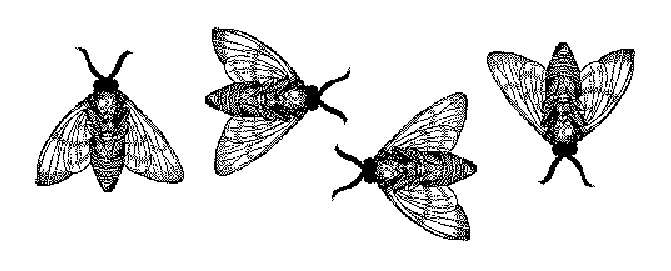
\includegraphics{flies}
\caption{A sample black and white graphic
that needs to span two columns of text.}
\end{figure*}


\begin{figure}
\centering

\includegraphics[height=1in, width=1in]{rosette}
\caption{A sample black and white graphic that has
been resized with the \texttt{includegraphics} command.}
\vskip -6pt
\end{figure}

\subsection{Theorem-like Constructs}
Other common constructs that may occur in your article are
the forms for logical constructs like theorems, axioms,
corollaries and proofs.  There are
two forms, one produced by the
command \texttt{{\char'134}newtheorem} and the
other by the command \texttt{{\char'134}newdef}; perhaps
the clearest and easiest way to distinguish them is
to compare the two in the output of this sample document:

This uses the \textbf{theorem} environment, created by
the\linebreak\texttt{{\char'134}newtheorem} command:
\newtheorem{theorem}{Theorem}
\begin{theorem}
Let $f$ be continuous on $[a,b]$.  If $G$ is
an antiderivative for $f$ on $[a,b]$, then
\begin{displaymath}\int^b_af(t)dt = G(b) - G(a).\end{displaymath}
\end{theorem}

The other uses the \textbf{definition} environment, created
by the \texttt{{\char'134}newdef} command:
\newdef{definition}{Definition}
\begin{definition}
If $z$ is irrational, then by $e^z$ we mean the
unique number which has
logarithm $z$: \begin{displaymath}{\log e^z = z}\end{displaymath}
\end{definition}

Two lists of constructs that use one of these
forms is given in the
\textit{Author's  Guidelines}.

There is one other similar construct environment, which is
already set up
for you; i.e. you must \textit{not} use
a \texttt{{\char'134}newdef} command to
create it: the \textbf{proof} environment.  Here
is a example of its use:
\begin{proof}
Suppose on the contrary there exists a real number $L$ such that
\begin{displaymath}
\lim_{x\rightarrow\infty} \frac{f(x)}{g(x)} = L.
\end{displaymath}
Then
\begin{displaymath}
l=\lim_{x\rightarrow c} f(x)
= \lim_{x\rightarrow c}
\left[ g{x} \cdot \frac{f(x)}{g(x)} \right ]
= \lim_{x\rightarrow c} g(x) \cdot \lim_{x\rightarrow c}
\frac{f(x)}{g(x)} = 0\cdot L = 0,
\end{displaymath}
which contradicts our assumption that $l\neq 0$.
\end{proof}

Complete rules about using these environments and using the
two different creation commands are in the
\textit{Author's Guide}; please consult it for more
detailed instructions.  If you need to use another construct,
not listed therein, which you want to have the same
formatting as the Theorem
or the Definition\cite{salas:calculus} shown above,
use the \texttt{{\char'134}newtheorem} or the
\texttt{{\char'134}newdef} command,
respectively, to create it.


\bibliographystyle{abbrv}
\bibliography{sigproc}

\end{document}
